\chapter{Corps purs et mélanges}\label{ch:g6:pure-substances-and-mixtures}

Une bouteille d'eau minérale énumère sur son étiquette une douzaine de
substances dissoutes, avec leurs quantités en milligrammes par litre.
L'eau qui sort du purificateur d'un laboratoire n'en mentionne aucune.
Les deux sont limpides et incolores, les deux étanchent la soif --- et
pourtant une seule est ce qu'un chimiste appelle une eau pure. Ce
chapitre donne au mot «~pur~» son sens exact, et montre comment
distinguer un \omterm{def:g6:pure-substances-and-mixtures:pure-substance}{corps pur} d'un \omterm{def:g6:pure-substances-and-mixtures:mixture}{mélange} sans rien goûter.

\begin{recall}
\omterm{def:g2:mixing-and-dissolving:mix}{Mélanger}, c'est mettre des choses différentes ensemble~; un solide qui
\omterm{def:g2:mixing-and-dissolving:dissolve}{se dissout} dans l'eau laisse le liquide limpide, et ce liquide limpide
est une solution (\cref{ch:g2:mixing-and-dissolving}). On peut séparer
un \omterm{def:g6:pure-substances-and-mixtures:mixture}{mélange} par \omterm{def:g3:separating-mixtures:sieve}{tamisage}, \omterm{def:g3:separating-mixtures:decant}{décantation}, \omterm{def:g3:separating-mixtures:filter}{filtration} et \omterm{def:g3:separating-mixtures:evaporate}{évaporation}
(\cref{ch:g3:separating-mixtures}). Chaque matériau a des propriétés que
l'on peut tester~: dur ou mou, transparent ou non, il flotte ou il coule
(\cref{ch:g1:materials-around-us}).
\end{recall}

\section{Espèces chimiques et corps purs}

\begin{definition}[Espèce chimique]\label{def:g6:pure-substances-and-mixtures:species}
Une \emph{espèce chimique}\index{espece chimique@espèce chimique} est une sorte
particulière de substance, avec son propre nom et ses propres
propriétés~: l'eau, le sucre, le sel, l'oxygène, l'éthanol (l'alcool du
vin), le fer.
\end{definition}

\begin{definition}[Corps pur]\label{def:g6:pure-substances-and-mixtures:pure-substance}
Un \emph{corps pur}\index{corps pur} est constitué d'une seule \omterm{def:g6:pure-substances-and-mixtures:species}{espèce
chimique} et de rien d'autre~: l'eau distillée, un cristal de sucre, une
bague en or pur.
\end{definition}

\begin{definition}[Mélange]\label{def:g6:pure-substances-and-mixtures:mixture}
Un \emph{mélange}\index{melange@mélange} contient plusieurs \omterm{def:g6:pure-substances-and-mixtures:species}{espèces chimiques}.
L'\omterm{def:g4:air-a-mixture-of-gases:air}{air}, l'eau de mer, l'eau minérale, le lait, le granite et le jus
d'orange sont des mélanges.
\end{definition}

\begin{remark}[«~Pur~» dans la langue de tous les jours]\label{rem:g6:pure-substances-and-mixtures:everyday}
Une brique de «~pur jus d'orange~» signifie que rien n'a été ajouté au
jus. Pour un chimiste, ce jus reste un \omterm{def:g6:pure-substances-and-mixtures:mixture}{mélange}~: de l'eau, des sucres,
des acides, des vitamines, des colorants et des arômes, beaucoup
d'\omterm{def:g6:pure-substances-and-mixtures:species}{espèces chimiques}. Une «~eau pure de montagne~» est elle aussi un
\omterm{def:g6:pure-substances-and-mixtures:mixture}{mélange}~: de l'eau contenant des sels dissous.
\end{remark}

\begin{omfigure}
\begin{tikzpicture}[font=\small, level distance=1.55cm,
    box/.style={draw=omDef, fill=omDef!6, rounded corners=2pt, align=center,
      inner sep=4pt},
    level 1/.style={sibling distance=7.2cm},
    level 2/.style={sibling distance=3.6cm},
    edge from parent/.style={draw, thick, omDef, ->}]
  \node[box] {matière}
    child {node[box] {corps pur\\ \footnotesize une seule espèce chimique}
      child {node[box, draw=black!40, fill=white] {eau distillée,\\ sel, fer}}}
    child {node[box] {mélange\\ \footnotesize plusieurs espèces chimiques}
      child {node[box] {homogène\\ \footnotesize même aspect partout}
        child {node[box, draw=black!40, fill=white] {eau salée,\\ air}}}
      child {node[box] {hétérogène\\ \footnotesize parties visibles}
        child {node[box, draw=black!40, fill=white] {eau boueuse,\\ granite}}}};
\end{tikzpicture}

{\small Classer la matière. Les cases du bas donnent des exemples de
chaque sorte.}
\end{omfigure}

\section{Mélanges homogènes et hétérogènes}

\begin{definition}[Mélanges homogènes et hétérogènes]\label{def:g6:pure-substances-and-mixtures:homogeneous}
Un \omterm{def:g6:pure-substances-and-mixtures:mixture}{mélange} est un \emph{mélange homogène}\index{melange homogene@mélange homogène}
quand on ne peut pas distinguer ses différentes parties à l'œil nu, même
à la loupe~: il a le même aspect partout. C'est un
\emph{mélange hétérogène}\index{melange heterogene@mélange hétérogène} quand on peut voir au
moins deux parties différentes.
\end{definition}

\begin{example}[Quatre mélanges]\label{ex:g6:pure-substances-and-mixtures:four}
L'eau salée et l'\omterm{def:g4:air-a-mixture-of-gases:air}{air} sont homogènes~: on ne voit pas leurs parties.
L'huile sur l'eau est hétérogène~: deux couches. L'eau boueuse est
hétérogène~: des grains y flottent et se déposent. Le jus d'orange avec
pulpe est hétérogène~: on voit les morceaux de pulpe.
\end{example}

\begin{omfigure}
\begin{tikzpicture}[font=\small, scale=1.15]
  \pic[transform shape] at (0,0) {beaker={0.7}{omWater!80}};
  \node[anchor=north, align=center] at (0,-0.15) {eau salée~:\\ homogène};
  \pic[transform shape] at (2.6,0) {beaker={0.7}{omWater!80}};
  \fill[yellow!55!orange!60] (1.8,1.05) rectangle (3.4,1.4);
  \draw[omGlass, line width=0.7pt] (1.8,1.05) -- (1.8,1.4) (3.4,1.05) -- (3.4,1.4);
  \node[anchor=north, align=center] at (2.6,-0.15) {huile sur l'eau~:\\ hétérogène};
  \pic[transform shape] at (5.2,0) {beaker={0.7}{brown!25}};
  \foreach \x/\y in {4.6/0.3,4.9/0.7,5.3/0.5,5.6/1.0,5.0/1.1,5.4/0.2,5.8/0.6}
    \fill[brown!65] (\x,\y) circle (0.04);
  \fill[brown!60] (4.4,0) rectangle (6.0,0.12);
  \node[anchor=north, align=center] at (5.2,-0.15) {eau boueuse~:\\ hétérogène};
  \pic[transform shape] at (7.8,0) {beaker={0.7}{orange!45}};
  \foreach \x/\y in {7.3/0.35,7.6/0.8,8.0/0.5,8.3/1.0,7.7/1.15,8.2/0.25,7.45/0.65}
    \fill[orange!80!brown] (\x,\y) ellipse (0.08 and 0.03);
  \node[anchor=north, align=center] at (7.8,-0.15) {jus avec pulpe~:\\ hétérogène};
\end{tikzpicture}

{\small Un \omterm{def:g6:pure-substances-and-mixtures:homogeneous}{mélange homogène} et trois \omterm{def:g6:pure-substances-and-mixtures:homogeneous}{mélanges hétérogènes}.}
\end{omfigure}

\begin{omfigure}
\begin{minipage}[b]{0.48\linewidth}\centering
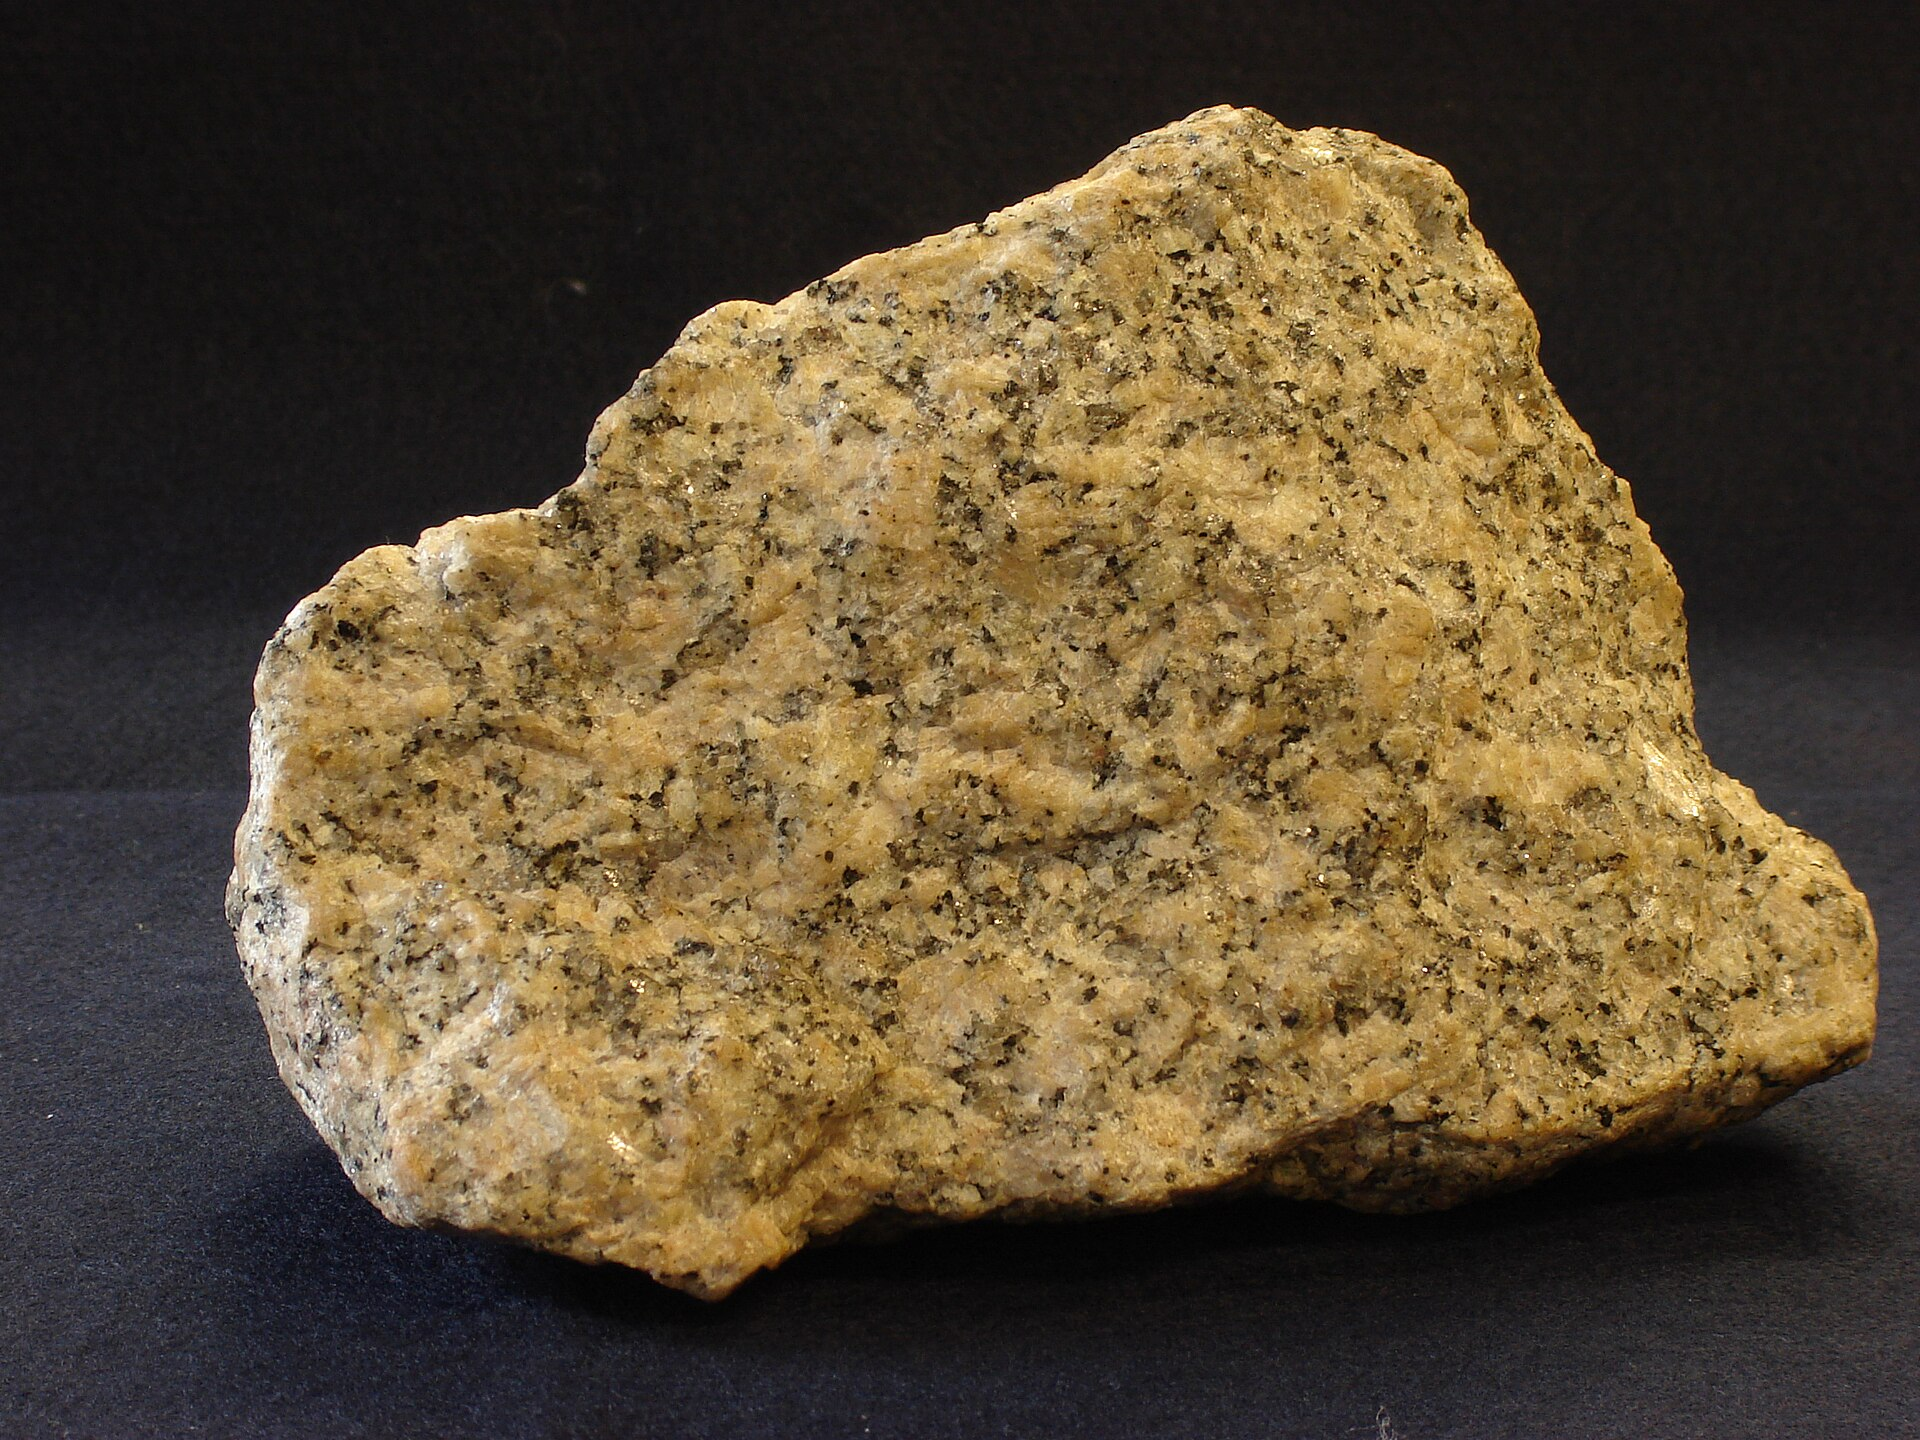
\includegraphics[width=\linewidth,height=4.6cm,keepaspectratio]{images/book1/granite.jpg}

{\small Le granite~: on y voit des grains de trois ou quatre minéraux
différents. Un solide hétérogène. Photo~: Eurico Zimbres, CC BY-SA 2.0 br.}
\end{minipage}\hfill
\begin{minipage}[b]{0.48\linewidth}\centering
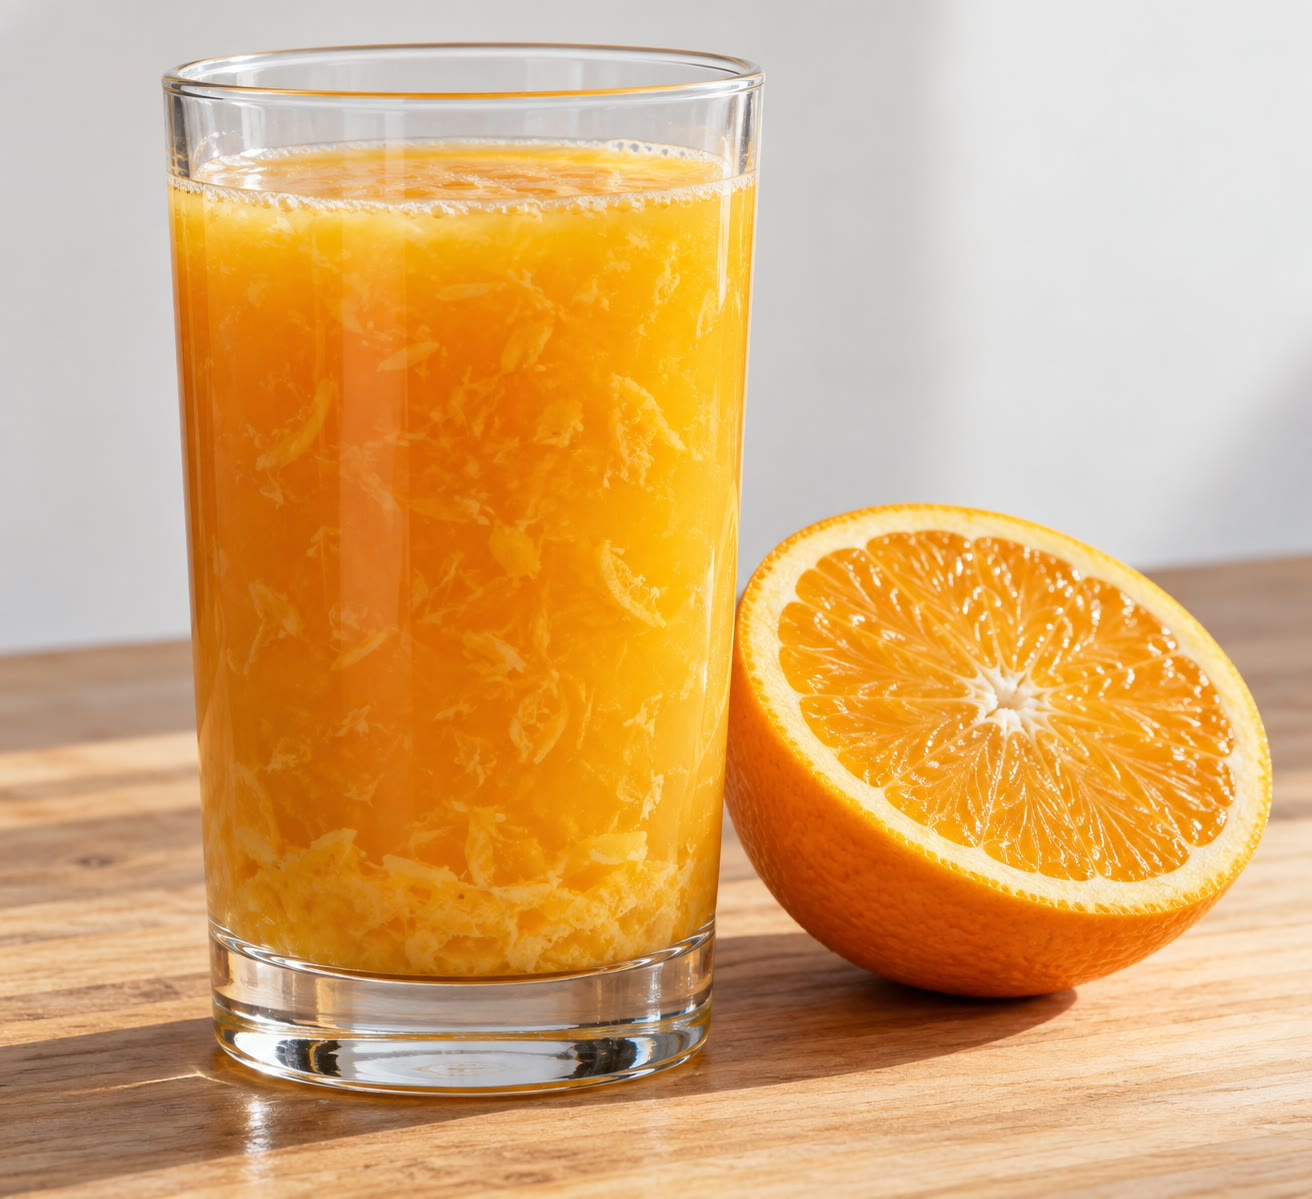
\includegraphics[width=\linewidth,height=4.6cm,keepaspectratio]{images/book1/ai/g6-orange-juice.jpg}

{\small Du jus d'orange avec pulpe~: un \omterm{def:g6:pure-substances-and-mixtures:homogeneous}{mélange hétérogène}.}
\end{minipage}
\end{omfigure}

\begin{remark}[Homogène ne veut pas dire pur]\label{rem:g6:pure-substances-and-mixtures:not-pure}
L'eau salée ressemble exactement à de l'eau pure. Regarder ne suffit pas
pour distinguer un \omterm{def:g6:pure-substances-and-mixtures:pure-substance}{corps pur} d'un \omterm{def:g6:pure-substances-and-mixtures:homogeneous}{mélange homogène}~: il faut mesurer
quelque chose.
\end{remark}

\section{Reconnaître un corps pur à ses constantes}

\begin{proposition}[Un corps pur a ses propres constantes]\label{prop:g6:pure-substances-and-mixtures:constants}
% ledger: mp:water, bp:water, bp:ethanol, mp:ethanol, rho:water, rho:ethanol, mp:NaCl, mp:Fe, rho:Fe
Chaque \omterm{def:g6:pure-substances-and-mixtures:pure-substance}{corps pur} fond à une température fixe qui lui est propre, bout à
une température fixe qui lui est propre (sous la pression normale), et a
sa propre masse pour un volume donné, sa masse volumique. Ces nombres
sont ses constantes~; le livre de physique explique ce qu'elles
mesurent. Pour quelques \omterm{def:g6:pure-substances-and-mixtures:pure-substance}{corps purs}~:
\begin{center}
\small
\begin{tabular}{lccc}
\hline
\omterm{def:g6:pure-substances-and-mixtures:pure-substance}{corps pur} & fond à & bout à & masse de \qty{1}{cm^3} \\
\hline
eau & \qty{0}{\celsius} & \qty{100}{\celsius} & environ \qty{1.0}{g} \\
éthanol & \qty{-114}{\celsius} & \qty{78}{\celsius} & \qty{0.79}{g} \\
propanone (acétone) & --- & \qty{56}{\celsius} & \qty{0.78}{g} \\
sel (chlorure de sodium) & \qty{801}{\celsius} & --- & \qty{2.17}{g} \\
fer & \qty{1538}{\celsius} & --- & \qty{7.87}{g} \\
\hline
\end{tabular}
\end{center}
% ledger: bp:acetone, rho:acetone, rho:NaCl
\end{proposition}

\begin{proposition}[Un mélange n'a pas de température d'ébullition fixe]\label{prop:g6:pure-substances-and-mixtures:mixture-boils}
Un \omterm{def:g6:pure-substances-and-mixtures:mixture}{mélange} ne bout pas à une température fixe~: l'eau salée commence à
bouillir un peu au-dessus de \qty{100}{\celsius}, et sa température
continue de monter pendant l'ébullition, car l'eau s'en va et le sel
qui reste devient plus concentré.
\end{proposition}

\begin{method}[Ce liquide est-il pur~? Lequel est-ce~?]\label{met:g6:pure-substances-and-mixtures:identify}
\begin{enumerate}
  \item Le chauffer, au laboratoire, et lire sa température pendant
        l'ébullition.
  \item Si la température reste fixe, le liquide est probablement un
        \omterm{def:g6:pure-substances-and-mixtures:pure-substance}{corps pur}~: comparer cette température à une table de constantes.
  \item Si la température continue de monter, c'est un \omterm{def:g6:pure-substances-and-mixtures:mixture}{mélange}.
  \item Confirmer avec une deuxième constante, par exemple la masse d'un
        volume connu.
\end{enumerate}
\end{method}

\begin{inthelab}[Faire bouillir de l'eau salée]
L'enseignant chauffe côte à côte de l'eau pure et de l'eau salée, avec
un thermomètre dans chacune. L'eau pure bout à \qty{100}{\celsius} et y
reste tant qu'elle bout. L'eau salée commence à bouillir un peu
au-dessus de \qty{100}{\celsius}, et le thermomètre monte lentement,
minute après minute.
\end{inthelab}

\section{L'eau, pure ou non}

\begin{example}[Quatre eaux]\label{ex:g6:pure-substances-and-mixtures:waters}
% ledger: sea:salinity
\begin{itemize}
  \item L'\textbf{eau distillée}, préparée au laboratoire, est presque un
        \omterm{def:g6:pure-substances-and-mixtures:pure-substance}{corps pur}~: de l'eau et rien d'autre.
  \item L'\textbf{eau du robinet} est un \omterm{def:g6:pure-substances-and-mixtures:homogeneous}{mélange homogène}~: de l'eau avec
        de petites quantités de substances dissoutes (une goutte séchée
        sur une assiette sombre laisse un cercle blanc).
  \item L'\textbf{eau minérale} est un \omterm{def:g6:pure-substances-and-mixtures:homogeneous}{mélange homogène} dont l'étiquette
        indique les substances dissoutes, en milligrammes par litre.
  \item L'\textbf{eau de mer} est un \omterm{def:g6:pure-substances-and-mixtures:homogeneous}{mélange homogène} qui contient
        environ \qty{35}{g} de sels par kilogramme.
\end{itemize}
\end{example}

\begin{omfigure}
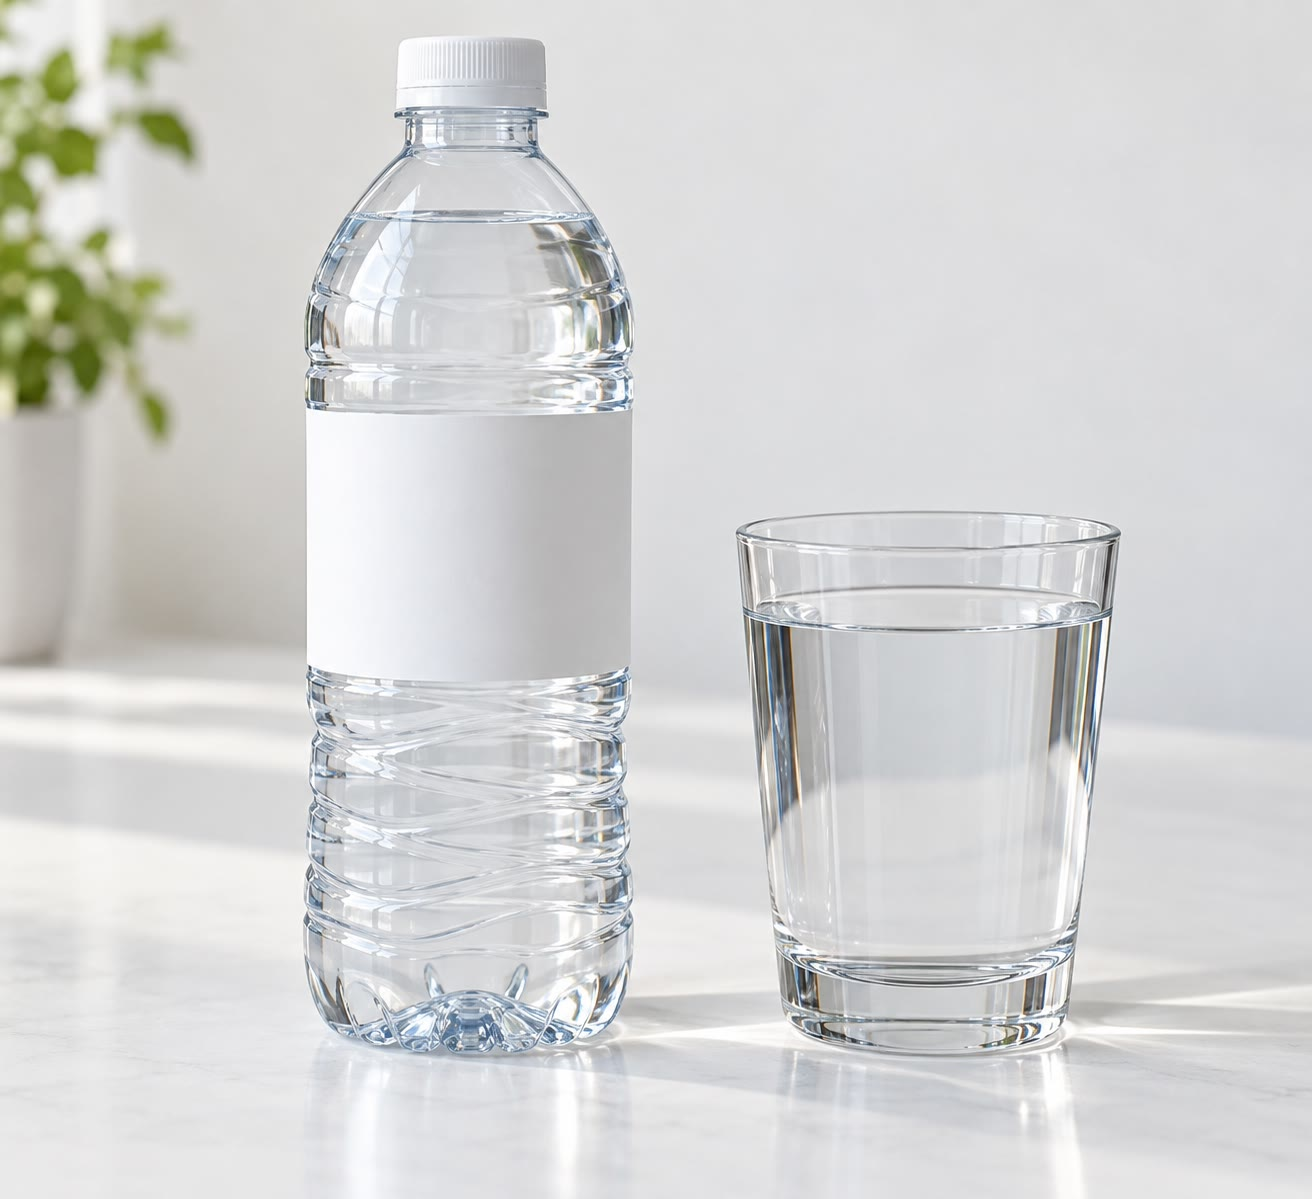
\includegraphics[width=0.5\linewidth]{images/book1/ai/g6-mineral-water.jpg}

{\small Une bouteille d'eau minérale~: limpide et incolore, et pourtant
un \omterm{def:g6:pure-substances-and-mixtures:mixture}{mélange}.}
\end{omfigure}

\begin{example}[Lire l'étiquette d'une eau minérale]\label{ex:g6:pure-substances-and-mixtures:label}
Une étiquette indique~: calcium \qty{78}{mg/L}, magnésium
\qty{24}{mg/L}, sodium \qty{5}{mg/L}, hydrogénocarbonate
\qty{357}{mg/L}, sulfate \qty{10}{mg/L}, chlorure \qty{4}{mg/L}. (Ces
valeurs sont un exemple.) Un litre contient
$78 + 24 + 5 + 357 + 10 + 4 = 478$\,mg de substances dissoutes, environ
un demi-gramme~: très peu à côté des \qty{1000}{g} d'eau, mais assez
pour en faire un \omterm{def:g6:pure-substances-and-mixtures:mixture}{mélange}.
\end{example}

\section{Exercices}

\begin{exercise}[$\star$]\label{exo:g6:pure-substances-and-mixtures:1}
\omterm{def:g6:pure-substances-and-mixtures:pure-substance}{Corps pur} ou \omterm{def:g6:pure-substances-and-mixtures:mixture}{mélange}~? L'eau distillée, l'\omterm{def:g4:air-a-mixture-of-gases:air}{air}, l'eau de mer, un bloc de
fer pur, le lait, un cristal de sucre.
\end{exercise}

\begin{exercise}[$\star$]\label{exo:g6:pure-substances-and-mixtures:2}
Homogène ou hétérogène~? L'eau salée, le granite, l'huile sur l'eau,
l'eau du robinet, le muesli.
\end{exercise}

\begin{exercise}[$\star$]\label{exo:g6:pure-substances-and-mixtures:3}
Qu'est-ce qu'une \omterm{def:g6:pure-substances-and-mixtures:species}{espèce chimique}~? Donne trois exemples.
\end{exercise}

\begin{exercise}[$\star$]\label{exo:g6:pure-substances-and-mixtures:4}
Un liquide bout à \qty{78}{\celsius}, et sa température reste à
\qty{78}{\celsius} pendant l'ébullition. À l'aide de la table des
constantes, propose une identité pour ce liquide.
\end{exercise}

\begin{exercise}[$\star$]\label{exo:g6:pure-substances-and-mixtures:5}
Pourquoi un «~pur jus d'orange~» n'est-il pas un \omterm{def:g6:pure-substances-and-mixtures:pure-substance}{corps pur} pour un
chimiste~?
\end{exercise}

\begin{exercise}[$\star\star$]\label{exo:g6:pure-substances-and-mixtures:6}
Un liquide commence à bouillir à \qty{100.5}{\celsius} et sa température
monte pendant l'ébullition. Est-ce un \omterm{def:g6:pure-substances-and-mixtures:pure-substance}{corps pur}~? Que pourrait-il être~?
\end{exercise}

\begin{exercise}[$\star\star$]\label{exo:g6:pure-substances-and-mixtures:7}
Regarde la figure des quatre béchers. Dans quel bécher un filtre
pourrait-il séparer les parties du \omterm{def:g6:pure-substances-and-mixtures:mixture}{mélange}~? Dans quel bécher ne le
pourrait-il pas~?
\end{exercise}

\begin{exercise}[$\star\star$]\label{exo:g6:pure-substances-and-mixtures:8}
Un cube de métal de volume \qty{10}{cm^3} a une masse de \qty{78.7}{g}.
Quelle est la masse de \qty{1}{cm^3}~? De quel métal de la table
pourrait-il s'agir~?
\end{exercise}

\begin{exercise}[$\star\star$]\label{exo:g6:pure-substances-and-mixtures:9}
D'après l'étiquette d'eau minérale de l'exemple, quel pourcentage de la
masse dissoute est de l'hydrogénocarbonate~? Arrondis à l'unité.
\end{exercise}

\begin{exercise}[$\star\star$]\label{exo:g6:pure-substances-and-mixtures:10}
L'eau de mer contient environ \qty{35}{g} de sels par kilogramme. Quelle
masse de sels y a-t-il dans un seau de \qty{2}{kg} d'eau de mer~? Quel
pourcentage de la masse de l'eau de mer est du sel~?
\end{exercise}

\begin{exercise}[$\star\star\star$]\label{exo:g6:pure-substances-and-mixtures:11}
Deux liquides limpides et incolores ont l'air identiques. Décris deux
mesures, faites au laboratoire, qui montreraient s'il s'agit du même
\omterm{def:g6:pure-substances-and-mixtures:pure-substance}{corps pur}.
\end{exercise}

\begin{exercise}[$\star\star\star$]\label{exo:g6:pure-substances-and-mixtures:12}
Un \omterm{def:g6:pure-substances-and-mixtures:mixture}{mélange} est fait de \qty{90}{g} d'eau et de \qty{10}{g} d'éthanol.
Quel pourcentage de sa masse est de l'éthanol~? Peut-on l'identifier
avec la table des constantes~? Explique.
\end{exercise}

\section{Problème~: trois liquides incolores}

\begin{problem}[{Problème du week-end --- trois flacons sans étiquette,
pleins d'un liquide limpide et incolore, et les mesures qui les
distinguent}]
\label{pb:g6:pure-substances-and-mixtures:1}
% ledger: bp:water, bp:ethanol, rho:water, rho:ethanol, rho:seawater, sea:salinity
Un assistant de laboratoire trouve trois flacons, A, B et C, dont les
étiquettes sont tombées. Tous les trois contiennent un liquide limpide
et incolore. Le laboratoire n'utilise que trois liquides de ce genre~:
de l'eau distillée, de l'éthanol, et de l'eau de mer rapportée d'une
sortie sur le terrain. L'assistant fait trois sortes de mesures, au
laboratoire.

\medskip
\noindent\textbf{Partie I --- Observer.}
\begin{enumerate}
  \item Les trois liquides ont exactement le même aspect. L'assistant
        peut-il savoir, en les regardant, lesquels sont des \omterm{def:g6:pure-substances-and-mixtures:pure-substance}{corps purs}~?
        Explique.
  \item Si l'un d'eux est un \omterm{def:g6:pure-substances-and-mixtures:mixture}{mélange}, est-il homogène ou hétérogène~?
  \item Quelle sorte de mesure peut montrer qu'un liquide est un \omterm{def:g6:pure-substances-and-mixtures:pure-substance}{corps
        pur}~?
\end{enumerate}

\medskip
\noindent\textbf{Partie II --- Mesurer.}
On chauffe chaque liquide jusqu'à l'ébullition. Le liquide A bout à
\qty{100}{\celsius} et sa température y reste. Le liquide B bout à
\qty{78}{\celsius} et y reste. Le liquide C commence à bouillir à
\qty{100.6}{\celsius}, et sa température continue de monter lentement.
On pèse ensuite \qty{50.0}{mL} de chaque liquide~: A \qty{49.8}{g}, B
\qty{39.5}{g}, C \qty{51.2}{g}.
\begin{enumerate}[resume]
  \item Quels liquides sont des \omterm{def:g6:pure-substances-and-mixtures:pure-substance}{corps purs}~? Lequel est un \omterm{def:g6:pure-substances-and-mixtures:mixture}{mélange}~?
  \item À l'aide de la table des constantes de ce chapitre, nomme les
        liquides A et B.
  \item Calcule la masse de \qty{1}{mL} (c'est-à-dire \qty{1}{cm^3}) de
        chaque liquide.
  \item Ces masses sont-elles en accord avec ta réponse à la question 5~?
  \item Pourquoi la température du liquide C continue-t-elle de monter
        pendant l'ébullition~?
\end{enumerate}

\medskip
\noindent\textbf{Partie III --- Que contient le liquide C~?}
On laisse sécher \qty{100}{mL} du liquide C dans une coupelle. Quand
toute l'eau est partie, il reste \qty{3.5}{g} de cristaux blancs.
\begin{enumerate}[resume]
  \item Que montre ce résidu au sujet du liquide C~?
  \item À l'aide de la masse de \qty{1}{mL} de C trouvée à la question 6,
        calcule la masse de \qty{100}{mL} de C, puis le pourcentage de sa
        masse qui est du sel (au dixième près).
  \item L'eau de mer contient environ \qty{35}{g} de sels par kilogramme.
        Quel pourcentage cela représente-t-il~? Compare avec la
        question~10.
  \item Conclus~: combien de grammes de sel chaque litre du liquide C
        contient-il, et le liquide C est-il l'eau de mer~?
\end{enumerate}
\end{problem}
